%17/10 - Óscar
\chapter{Acceso programático a bases de datos biomédicas}
\section{Introducción}
En este bloque queremos acceder mediante los programas a las bases de datos biomédicas y poder interactuar con ellas. Para las bases de datos biomédicas hay que hacer peticiones desde el protocolo HTTP. Un protocolo es una forma de interacción entre dos partes: queremos hacer una petición a la base de datos a partir de una entrada para que nos devuelva una respuesta que podamos utilizar posteriormente. Tenemos que usar los protocolos intermediarios para poder interactuar con la base de datos. Como esto puede ser un lío, se diseñaron las API REST. Un API es application programming interface, es decir, un protocolo o una manera de interactuar con otra parte en un formato concreto. REST tiene que ver con el protocolo HTTP de base. El protocolo HTTP se utiliza para navegar por internet. Muchas aplicaciones exponen un API REST, lo que quiere decir que hay unas ciertas órdenes o funciones que se pueden llamar para interactuar con la aplicación. Hay una serie de endpoints, que son cada una de las funciones que están disponibles para llamar: un endpoint para buscar un organismo concreto, para descargar una cierta secuencia, etc. 

Hay varias maneras de acceder a bases de datos en línea (nivel de abstracción o automatización ascendente):
\begin{itemize}
\item \textbf{Copiar la base de datos de manera local}: esto es un proceso manual que hace que la base de datos se quede rápidamente desactualizada. Se puede descargar un fichero de un servicio web en Linux mediante \texttt{wget url/base/de/datos/fichero.txt}
\item \textbf{Rellenar formularios}: todavía el sistema no ha dado acceso al público a sus servicios mediante API, pero se puede escribir en Python un programa que rellene el formulario como si fuera un humano para acceder a los datos cambiando los valores de los parámetros. En general, la sintaxis de una URL es la siguiente:
\begin{center}
scheme:[//host]path[?query][\#fragment]\\
\end{center}
siendo scheme HTTP o HTTPS cuando el protocolo está cifrado y es seguro (la s viene de secure), host el servidor que contiene la base de datos a la que se quiere acceder, el path la ruta para llegar a una parte del servidor (como si fueran carpetas) y la interrogración el marcador de los argumentos (las queries se escriben en formato nombre=valor\&nombre2=valor2). Así, lo que queremos hacer con Python es codificar los distintos argumentos para poder acceder a varias entradas de forma automática. Por ejemplo, en el formulario tipo \href{https://www.ebi.ac.uk/Tools/dbfetch/dbfetch?db=ena\_sequence\&id=J00231\&style=raw}{https://www.ebi.ac.uk/Tools/dbfetch/dbfetch?db=ena\_sequence\&id=J00231\&style=raw}, en lugar de rellenar el formulario varias veces, queremos cambiar el valor de los distintos argumentos (id=J00231, id=J00232, id=J00233, db=afdb, etc.). 
\item \textbf{Peticiones HTTP directas:} esto se puede conseguir mediante la librería \texttt{requests} en Python o mediante la terminal. Se emplean las URLs de los distintos servidores con métodos como GET y POST.
\item \textbf{Uso específico de API REST:} Hay algunos servicios que proporcionan APIs de los servidores para poder utilizarlos desde Python. Esto se conoce como APIs de alto nivel o SDKs. Esta es la mejor manera, ya que es más cómoda y más fácil de utilizar, pero no está disponible en todos los sistemas. Estas API REST están muy encapsuladas, por lo que no disponen de URLs ni GET o POST.
\end{itemize} 

\subsection{Acceso programático en formularios}
Hay varias librerías disponibles en Python para automatizar el acceso y procesado de las URL:
\begin{itemize}
\item \texttt{urllib}: acceso de bajo nivel, más adecuado para programación de red.
\item \texttt{requests}
\end{itemize}

La librería requests tiene el comando \texttt{get}, que es el método HTTP más común. 
\begin{lstlisting}[language=Python]
import requests
url = "https://www.ebi.ac.uk/Tools/dbfetch/dbfetch?db=ena_sequence&id=J00231&style=raw"
response = requests.get(url)
print(response.text)
\end{lstlisting}

En el método \texttt{get} de requests se puede utilizar el argumento \texttt{params} para pasar los distintos argumentos. Este argumento debe ser un diccionario con los distintos parámetros:
\begin{lstlisting}[language=Python]
import requests

ebi_url = 'https://www.ebi.ac.uk/Tools/dbfetch/dbfetch'

response = requests.get(ebi_url,
    params={'db': 'ena_sequence', 'id':'J00231' , 'style':'raw'})

print(response.text)
\end{lstlisting}

\section{JSON}
Hay distintas formas de poder representar un fichero:
\begin{itemize}
\item Texto plano
\item HTML (HyperText Markup Language)
\item XML (eXtensible Markup Language)
\item JSON (JavaScript Object Notation)
\end{itemize}

La notación JSON es similar a la de los diccionarios en Python conceptualmente: las claves son strings y los valores pueden ser strings, números, listas o incluso diccionarios. Técnicamente es una forma de estructurar la información (figura \ref{fig:json}) en formato ASCII. 

\begin{figure}[htbp]
\centering
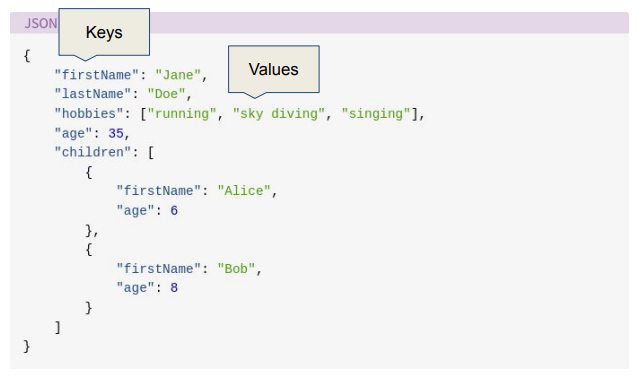
\includegraphics[width = 0.7\textwidth]{figs/json.png}
\caption{Ejemplo de un fichero JSON que describe a una persona. Las llaves representan estructuras y los corchetes listas.}
\label{fig:json}
\end{figure}

Python cuenta con una librería llamada \texttt{json}.
\begin{lstlisting}[language=Python]
import json

json_data =  '{"name":"John", "age":30, "city":"New York"}'

print(json_data)
\end{lstlisting}

%22/10 - Óscar
Para cargar un JSON, se utiliza el método \texttt{json.loads()}. Así, el JSON se guarda en un diccionario que posteriormente se puede guardar serializado en disco. Otra función es \texttt{json.dumps()}, el cual coge un diccionario en una cadena tipo JSON. La función \texttt{json.dump} escribe un objeto JSON en un fichero. 

\begin{table}[htbp]
\centering
\begin{tabular}{l | l}
dict = json.loads(str) & Convierte un string en un diccionario \\
str = json.dumps(dict) & Convierte un diccionario en un string \\
json.dump(dict, file) & Escribe un objeto JSON (dict) en un fichero
\end{tabular}
\caption{Resumen}
\end{table}

\section{Protocolo HTTP}
Los protocolos de acceso a las bases de datos se han montado sobre el protocolo HTTP. HTTP es un protocolo para obtener recursos en la web, como documentos HTML, imágenes y otros. Es un \textbf{protocolo cliente-servidor}, lo que significa que las peticiones las inicia el destinatario, normalmente el navegador web. 

Una página web es una colección de recursos: imágenes, vídeos, anuncios, etc. Estos elementos pueden estar en sitios distintos, y cuando la página se carga, se embebe en el código y se muestra.
\begin{figure}[htbp]
\centering
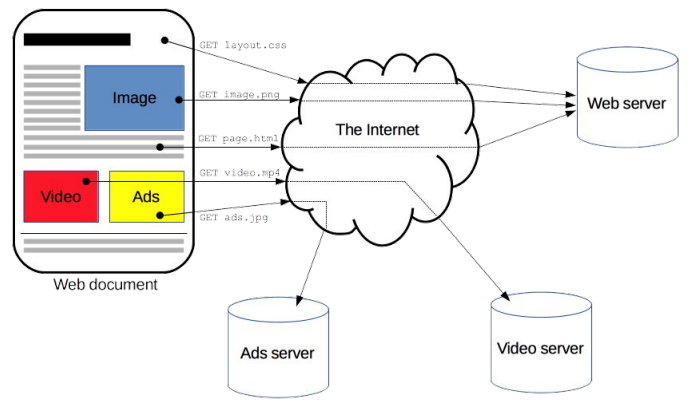
\includegraphics[width = 0.8\textwidth]{figs/web-http.png}
\end{figure}

Los clientes y los servidores se comunican intercambiando mensajes individuales (a diferencia de un flujo de datos). Los mensajes enviados por el cliente, normalmente un navegador web, se denominan \textbf{peticiones (requests)} y los mensajes enviados por el servidor como respuesta se denominan \textbf{respuestas (responses)}.

\subsection{Aspectos básicos de HTTP}
HTTP se diseñó para ser sencillo y legible para los humanos. Los mensajes HTTP pueden ser leídos y comprendidos por humanos, lo que facilita las pruebas a los desarrolladores y reduce la complejidad para los recién llegados. Además, HTTP es extensible: Las cabeceras HTTP hacen que este protocolo sea fácil de ampliar y experimentar. Se pueden introducir nuevas funciones mediante un simple acuerdo entre un cliente y un servidor sobre la semántica de una nueva cabecera.

HTTP no tiene estado, es decir, no existe ningún vínculo entre dos solicitudes que se realizan sucesivamente en la misma conexión. Las cookies HTTP permiten el uso de sesiones con estado (por ejemplo, para utilizar cestas de la compra de comercio electrónico).

\subsection{Flujo HTTP}
Cuando un cliente quiere comunicarse con un servidor realiza los siguientes pasos: 
\begin{enumerate}
\item Abre una conexión TCP: la conexión se utiliza para enviar una petición, o varias, y recibir una respuesta.
\item Envía un mensaje HTTP
\item Espera una respuesta
\end{enumerate}
\begin{figure}[htbp]
\centering
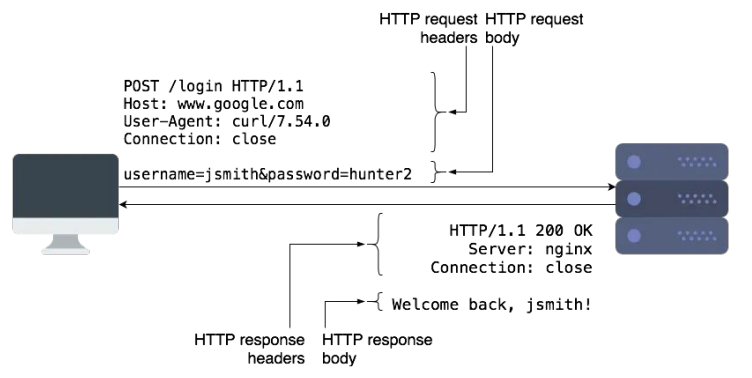
\includegraphics[width = 0.8\textwidth]{figs/http-flow.png}
\end{figure}

Las peticiones son puro texto (no hay datos binarios). La estructura es la siguiente: verbo, url y cabecera para proporcionar información adicional (por ejemplo, el idioma de una página web). La respuesta contiene una línea inicial con el HTTP y un código asociado (200 si todo está bien, 404 si no se ha encontrado, etc), la cabecera y el cuerpo.
\begin{figure}[htbp]
\centering
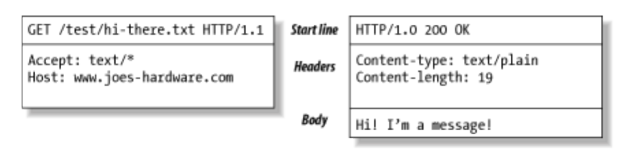
\includegraphics[width = 0.6\textwidth]{figs/request-answer.png}
\end{figure}

Los códigos de retorno son los siguientes:
\begin{table}[htbp]
\centering
\begin{tabular}{c | c | c}
Rango disponible & Rango definido & Categoría \\ \hline
100-199 & 100-101 & Información \\
200-299 & 200-206 & Éxito \\
300-399 & 300-305 & Redirección \\
400-499 & 400-415 & Error del cliente \\
500-599 & 500-505 & Error del servidor 
\end{tabular}
\caption{Códigos de retorno}
\end{table}

Un servidor es un ordenador en un data center. Cada servicio tiene asignado un puerto, ya que en un mismo servidor puede haber varios servicios web. Las direcciones IP (técnicamente IPv4) se dividen en cuatro bloques de tres números que van del 0 al 255 (esto ocupa 8 bites). Así, en el mundo puede haber un máximo de $255^4$ direcciones IP en el mundo. Por ello, a los servicios se les añade después de la dirección IP el puerto. En el caso de la web de la UAM, se trata de 150.244.214.237:80 para HTTP y 150.244.214.237:443 para HTTPS. Todos los servicios seguros (HTTPS) se conectan al puerto 443. Una vez conectados al servidor, se puede utilizar el método \texttt{GET} para obtener como respuesta la web que se está pidiendo. Esto se puede realizar en Python con la librería requests y la función get, como se explicó anteriormente. También está el método \texttt{POST} para enviar datos o información a un servidor. Estos datos se incluyen en el cuerpo de la petición, no están visibles en la URL, por lo que se suele utilizar para los login al ser más seguro (usuario y contraseña está oculto a la vista). En resumen: se pide información con GET y se envía información con POST. 

\textbf{Ejemplo: \href{https://rest.ensembl.org/}{https://rest.ensembl.org/}}
Aquí se pueden ver todos los endpoints (las distintas funcionalidades) de la página Ensembl. 
Con \texttt{GET archive/id/:id} se puede acceder a la última versión del identificador que se dé. :id indica la variable que se debería proporcionar, es decir, sustituirlo con el ID. Lo que se devuelve está en formato JSON, pero al leerlo en Python será del tipo string. En este ejemplo, hay un endpoint \texttt{POST archive/id} que lo que hace es devolver la última versión para un conjunto de identificadores. Antes hemos dicho que POST se utiliza para enviar información y GET para obtenerla, pero esta API está mal diseñada y diferencia GET y POST en que el primero es para un solo identificador y el segundo para varios.

En esta página se proponen ejemplos de peticiones. Para GET sería la siguiente:
\begin{lstlisting}[language=Python]
import requests, sys
 
server = "https://rest.ensembl.org"
ext = "/archive/id/ENSG00000157764?"
 
r = requests.get(server+ext, headers={ "Content-type" : "application/json"})
 
if not r.ok:
  r.raise_for_status()
  sys.exit()
 
decoded = r.json() #sería mejor utilizar json.loads 
print(repr(decoded))
\end{lstlisting}

\subsection{APIs con HTTP}
Los métodos HTTP originales tienen la siguiente semántica:
\begin{itemize}
\item GET: pide obtener una representación del recurso identificado
\item POST: pide añadir información al recurso
\item HEAD: como GET, pero sin recibir el cuerpo, solo la cabecera
\item Otros verbos como DELETE, PUT, CONNECT, TRACE, etc.
\end{itemize}

Para nuestros fines, se utilizará casi siempre GET, pero algunos servidores de datos biomédicos también aceptan POST. Sin embargo, algunos servidores que aceptan POST no lo utilizan para el fin previsto (crear información en el servidor), sino sólo para responder con la representación del recurso (al igual que GET).
URLs como las siguientes utilizan el método GET: \\
\href{https://rest.ensembl.org/sequence/id/ENSG00000157764}{https://rest.ensembl.org/sequence/id/ENSG00000157764} \\
\href{https://www.ebi.ac.uk/Tools/dbfetch/dbfetch?db=uniprot\&id=WAP\_RAT}{https://www.ebi.ac.uk/Tools/dbfetch/dbfetch?db=uniprot\&id=WAP\_RAT}

Un método POST equivalente utiliza una URL sin parámetros (\href{http://rest.ensembl.org/sequence/id/}{http://rest.ensembl.org/sequence/id/}) que se deben enviar junto a los parámetros en el cuerpo de la petición ({"ids":["ENSG00000157764"]}).
\begin{lstlisting}[language=Python]
## GET ##
import requests
gene = "ENSG00000157764"
endpoint = f"http://rest.ensembl.org/sequence/id/{gene}"
r = requests.get(endpoint, headers={ "Content-Type" :"text/plain"})

#Especificando params
gene = "ENSG00000157764"
endpoint = f"http://rest.ensembl.org/sequence/id/{gene}"
parameters = {'species': 'homo_sapiens'}
r = requests.get(endpoint, params = parameters, headers={"Content-type" : "text/json"})

## POST ##
#Especificando data en lugar de params
response = requests.post(server, data = {'key':'value'})
\end{lstlisting}

\begin{figure}[htbp]
\centering
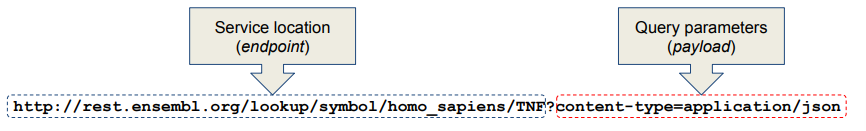
\includegraphics[width = \textwidth]{figs/rest-request.png}
\end{figure}

Aunque las bases de datos sean de acceso público (open access), usualmente piden una API Key, que es un número largo único para cada usuario registrado que se pone en la cabecera. De esa forma, proporcionando el API Key, el servidor sabe qué usuario se está conectando y puede limitar las peticiones de un mismo usuario.

\section{API REST}
REST viene de REpresentational State Transfer. Realmente no es un protocolo, si no un estilo de prestación de servicios web basados en HTTP. 
Los \textbf{servidores} aportan representaciones textuales de recursos (como XML, JSON o HTML), y los \textbf{clientes} piden servicios mediante los métodos HTTP (GET, POST, etc). 
El estado no se guarda en el servidor (cada petición se responde de forma independiente sin memoria de peticiones anteriores).

%24/10 - Óscar
\section{Examen de prueba}
\subsection{Ejercicio 1}
(1,5 puntos) Implementa una función write\_dna\_sequece que recupere de rest.ensembl.org y escriba en un fichero, cuyo nombre se reciba como parámetro, la secuencia ADN de un identificador dado. Adicionalmente, si se especifica un parámetro opcional a la función denominado ‘analysis’ y éste tiene el valor True, la función deben imprimir también por pantalla el número total de bases, así como el número de cada una de ellas. La salida debe ser similar a la siguiente: \\
File ‘dna\_sequence.txt' successfully written. \\
Total number of bases: 205603 \\
Number of 'A' bases: 60015 \\
Number of 'C' bases: 37965 \\
Number of 'G' bases: 40168 \\
Number of 'T' bases: 67455 \\
Para la implementación de la función, puedes utilizar el siguiente endpoint: \\
GET /sequence/id/:id recupera secuencias por identificador. \\
cuya documentación se muestra más abajo. No es necesario el uso de parámetros opcionales del endpoint.

\begin{figure}[htbp]
\centering
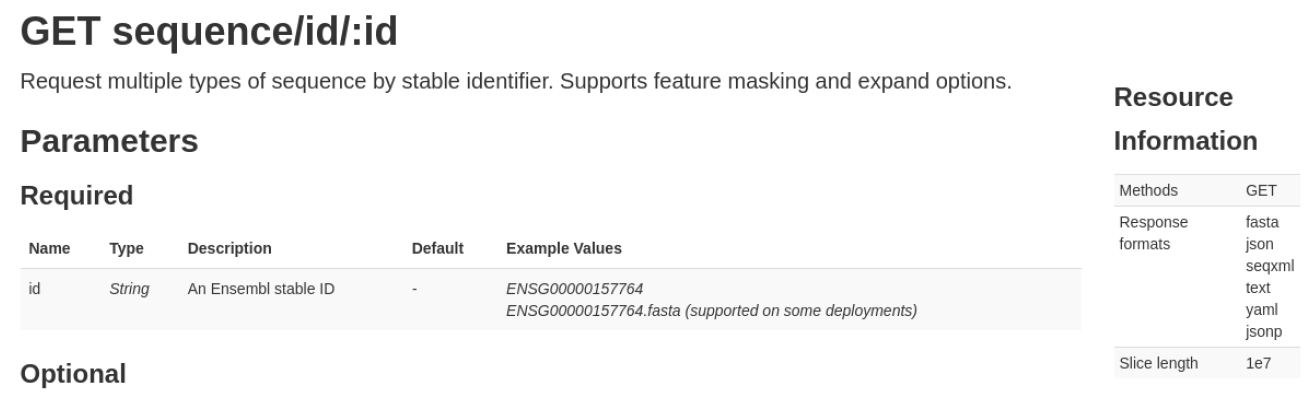
\includegraphics[width = \textwidth]{figs/endpoint-examen.png}
\caption{Documentación del endpoint}
\end{figure}

\begin{lstlisting}[language=Python]
import requests

def write_dna_sequence(DNA_id, file_name, analysis = False):
	"""Función que obtiene la secuencia de Ensembl y la escribe en un fichero.
	Input Parameters
	----------------------
	DNA_id: str
		ID de la secuencia que se quiere guardar
	file_name: str
		nombre del fichero en el que se quiere guardar la secuencia
	analysis: bool
		Parámetro que imprime la cantidad total de bases y el número de bases de cada nucleótido cuando True (por defecto).
		"""
	server = "rest.ensembl.org/"
	endpoint = f"sequence/id/{DNA_id}"
	
	response = requests.get(f"{server}{endpoint}", headers = {"Content-type":"application/text"})
	
	if response.ok:
		dna_sequence = response.text
		with open(file_out, "w") as f:
			f.write(dna_sequence)
		print(f"File {file_out} successfully written.")
		
		if analysis:
			print(f"Total number of bases: {len(dna_sequence)}")
			for nucleotide in "ATCG":
				print(f"Number of {nucleotide} bases: {dna_sequence.count(nucleotide)}")
	else:
		print("Se ha producido un error")
\end{lstlisting}

\subsection{Ejercicio 2}
(1 punto) El siguiente programa tiene como objetivo obtener la información de la versión más reciente de un gen específico. Desafortunadamente, no funciona como se espera. Señala y explica todos los errores, y escribe una versión corregida.
\begin{lstlisting}[language=Python]
import requests, sys, json
import pprint

server = "http://rest.ensembl.org"
gene = "ENSG00000157764"
get_gene_info_endpoint = f"/overlap/id/{gene}?feature=gene"
r = requests.get(f"{server}{get_gene_info_endpoint}")

if r.ok:
	r.raise_for_status()
	sys.exit()

pprint(r) 
\end{lstlisting}

Primero, la comprobación de la petición está invertida: cuando la petición se ha realizado correctamente, queremos continuar con el programa, y cuando ha habido algún error, se quiere apagar el sistema. Además, como importamos el módulo \texttt{pprint}, al llamar a una función dentro de ese módulo se debe utilizar la estructura módulo.función, no solo la función. Asimismo, como queremos imprimir el contenido de la petición, esto se encuentra dentro de text. Finalmente, se está importando el módulo json y no se está utilizando. Esto no es un error en sí, solo un warning, pero se puede reemplazar pprint con \texttt{json.loads(r.text)} y un print normal. Así, el código corregido quedaría de la siguiente forma:
\begin{lstlisting}[language=Python]
import requests, sys, json
import pprint

server = "http://rest.ensembl.org"
gene = "ENSG00000157764"
get_gene_info_endpoint = f"/overlap/id/{gene}?feature=gene"
r = requests.get(f"{server}{get_gene_info_endpoint}")

if not r.ok: #r.ok == False
	r.raise_for_status()
	sys.exit()

pprint.pprint(r.text)

##Alternativa
r_dict = json.loads(r.text)
print(r_dict)
\end{lstlisting}